\documentclass[thesis.tex]{subfiles}

\begin{document}
\chapter{Performance testing}
This chapter is concerned with testing the efficiency of the approach by running tests on the implemented tool. There are two metrics which will be presented: The running time of the algorithm and the correctness of the achieved result. How correctness is determined is covered in section \ref{sec:performance_validation}. Most of the results are compared against running the same alignment with an own PO-MSA implementation. PO-MSA is chosen because of its intuitive nature, the easily deducible relationship between graph complexity and running time and, most importantly, because it is a non-heuristical approach which means it guarantees a correct result every time.
\section{Test data}
These tests are meant to reflect usage in a what would be an every day situation, and does therefore use real genetic data. All of the sequences are FASTA-files from the MHC region, most fetched from the vg github repo\cite{vg}, some from the test-set provided by the sequence graphs tool\cite{sequence_graphs}. The exact test sets are chosen to provide a variety of sequence lengths. In order to cover lengths where we found no sequences there are created artificial sequences by cutting out suitable regions from longer sequences. All the sequences which are used can be found in the test-folder of the github repo of the tool (Appendix \ref{sec:tool}).\\
\par\noindent
Specifically, there are 8 main data-sets involved in the testing process:
\begin{itemize}
  \item \textbf{mhc1.fa} A 700 bp long sequence from the MHC region (not specified more precisely where). Fetched from the docker repo of the sg project
  \item \textbf{primary.fasta} A 3345 bp long sequence from the HLA-A gene in the MHC region from the primary assembly of GRCh38. Originates from the vg github.
  \item \textbf{20k.fasta, 35k.fasta, 100k.fasta, 150k.fasta, 500k.fasta} Five subsequences of an alternate assembly of the MHC region of respectively 21.070bp, 35.770bp, 101.570bp, 144.480bp and 448.490bp. The alternate assembly originates from the NCBI database\cite{ncbi} with id NT\_167244.1.
  \item \textbf{mhc\_full.fa} The previously mentioned full mhc assembly of 4.622.290bp.
\end{itemize}
Additionally, some of the tests use more specific data. This data will be presented when necessary. All the test data found can be found in the github repo\ref{tool}, in the data-folder\\
\par\noindent
In order to do alignments we needed reads aswell as the reference data itself. These reads are generated by the read-generator seen in the appendix. A read $r$ from a graph $G$ is generated by the following procedure:
\begin{enumerate}
  \item Choose a random vertice $v \in G\\\{s_G, t_G\}$ such that the smallest distance from $v$ to $t_g$ is larger than the chosen read size $|r|$
  \item For $r$ steps:
  \begin{enumerate}
    \item Append $b(v_x)$ to the read $r$
    \item Choose a random neighbouring vertice $v_y \in neighbours(v_x)$ as the new $v_x$
  \end{enumerate}
  \item When a read $r$ has been generated, for $r_i \in r$
  \begin{enumerate}
    \item Choose a random floating point value $0<=v<=1$
    \begin{itemize}
      \item If $v<(p/3)$ delete $r_i$
      \item Else if $v<(2p/3)$ insert a random base $b \in \{A, C, G, T\}$ before $r_i$
      \item Else if $v<p$ substitue $r_i$ with a random base $b \in \{A, C, G, T\} \\ \{r_i\}$
    \end{itemize}
  \end{enumerate}
  \item Output $r$
\end{enumerate}
In order to provide reproducability the randomness in the reads are generated from a seed.\\
\par\noindent
Because this thesis is concerned with the mathematical properties of the model the noise in the reads does not necessarily depict the true nature of either genetic variation (Section \ref{sec:genetic_variation}) or read errors (Section \ref{sec:sequencing}). This is acceptable because any specification of how alignments should be scored will be a specification of the general problem, and is thus left for others.
\section{Validation}
\label{sec:performance_validation}
When an alignment is produced for a read we classify it as either as correct or not correct. Intuitively one could imagine this can be figured out by determining whether the generated read aligns back to the path it was generated from. However, when noise is introduced an interesting phenomenon can occur: The modified read can be more similar to another path in the graph than its origin. This can also occur whenever there exists actual equal paths in the graph, typically in the case of repeats. In order to stick with mathemathical properties, our definition of optimality holds no relation to the origin of a read but is purely defined as the path which produces the highest possible alignment score. As PO-MSA is an exhaustive search we define optimally aligned as alignments which produce the same alignment score as the highest score found by PO-MSA. Consequently, as only the scores are compared, even when the approach produces a different alignments than PO-MSA this can be classified as optimal.\\
\par\noindent
\section{Time capturing mechanisms}
For both the "Fuzzy context-based search" and the PO-MSA algorithm the time capturing mechanisms are built into the tool, using the Java System object. This allowed us to wrap the time capturing of each individual constituent as close to the functional parts as possible in order to avoid unecessary overhead. When comparing tools the time was taken from the tool was started until the tool ended. Doing it this way has several disadvantages, which are discussed in Section \ref{sec:comparison_tools}.
\section{Building the index}
\begin{wraptable}{r}{0.5\textwidth}
  \begin{tabular}{|l|r|r|}
    \hline \textbf{Data set:} & \textbf{$|G|$} & \textbf{Time (ns)}\\ \hline
    mhc1.fa & 700 & 597127494\\ \hline
    primary.fasta & 3345 & 2050636347\\ \hline
    20k.fasta & 21070 & 13858701254\\ \hline
    30k.fasta & 35770 & 25401423058\\ \hline
    100k.fasta & 101570 & 77928851412\\ \hline
    150k.fa & 144480 & 122654330941\\ \hline
  \end{tabular}
  \caption{Runtimes of build\_index.sh}
\end{wraptable}
The building of the index is the first step of the process realized through the build\_index.sh script. To summarize this step consists of reading the input files, building the graph and generating the suffix trees. The build process was run 50 times on 6 different data sets, the averaged results can be seen in table \ref{tab:build_index}. All of these are linear operations which can be seen in \ref{build_index}.\\
\begin{figure}[!b]
    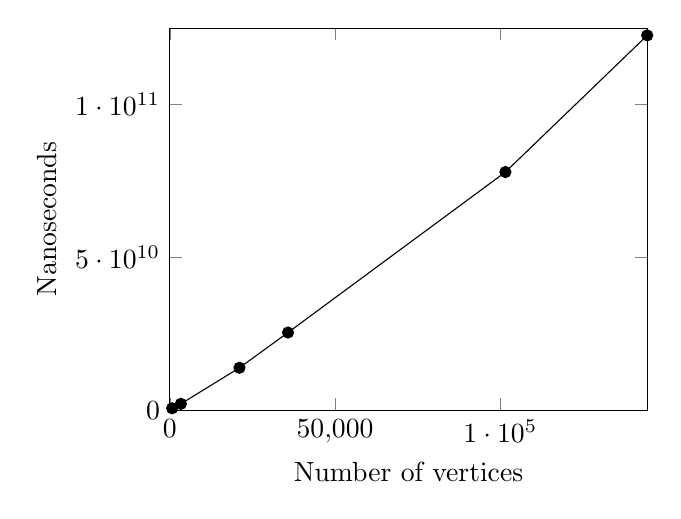
\begin{tikzpicture}
      \begin{axis}[scale only axis,height=0.4\textwidth,width=0.5\textwidth,xmin=0,ymin=0,xmax=144480,ymax=125000000000,scaled ticks=false, xlabel={Number of vertices}, ylabel={Nanoseconds}, max space between ticks=50pt]
        \addplot[color=black,mark=*] coordinates {
          (700,597127494)
          (3345,2050636347)
          (21070,13858701254)
          (35770,25401423058)
          (101570,77928851412)
          (144480,122654330941)
        };
      \end{axis}
    \end{tikzpicture}
    \caption{Runtime for the build index procedure}
    \label{fig:build_index}
\end{figure}
\noindent
When splitting up the runtime into the individual constituents an interesting pattern emerges (Fig. \ref{fig:index_constituents}): The main load of the indexation lies in writing to file. The data structure used is a large tree of nested complex structures such as hashmaps, which the standard Java serialization does not handle well \textcolor{red}{PROB SHUD REFERENCE SOMETHING. API MAYBE}. Putting effort into reducing the size of the index will thus have a dramatic effect on the time complexity.
\begin{figure}[!t]
  \begin{subfigure}[t]{0.4\textwidth}
    \begin{tikzpicture}[trim axis left]
      \begin{axis}[scale only axis,height=\textwidth,width=\textwidth,xmin=0,ymin=0,xmax=144480,ymax=122654330941,scaled ticks=false]
        \addplot coordinates {
          (700,9404263)
          (3345,51489024)
          (21070,623903806)
          (35770,1031820116)
          (101570,5487825644)
          (144480,11328920839)
        };
      \end{axis}
    \end{tikzpicture}
    \subcaption{Time used building the graph}
  \end{subfigure}
  \hfill
  \begin{subfigure}[t]{0.4\textwidth}
    \begin{tikzpicture}[trim axis left]
      \begin{axis}[scale only axis,height=\textwidth,width=\textwidth,xmin=0,ymin=0,xmax=144480,ymax=122654330941,scaled ticks=false]
        \addplot[color=green,mark=*] coordinates {
          (701,65184733)
          (3416,138556745)
          (21070,269431681)
          (35770,2788165703)
          (101570,6905517064)
          (144480,10007919085)
        };
      \end{axis}
    \end{tikzpicture}
    \subcaption{Time used building the index}
  \end{subfigure}
  \begin{subfigure}[b]{0.4\textwidth}
    \begin{tikzpicture}[trim axis left]
      \begin{axis}[scale only axis,height=\textwidth,width=\textwidth,xmin=0,ymin=0,xmax=144480,ymax=122654330941,scaled ticks=false]
        \addplot[color=red,mark=*] coordinates {
          (700,522174790)
          (3345,1860265733)
          (21070,1296505592)
          (35770,21581107294)
          (101570,65535179527)
          (144480,101317180800)
        };
      \end{axis}
    \end{tikzpicture}
    \subcaption{Time used writing the index\vspace{\baselineskip}}
  \end{subfigure}
  \hfill
  \begin{subfigure}[b]{0.4\textwidth}
  \begin{tikzpicture}[trim axis left]
    \begin{axis}[scale only axis,height=\textwidth,width=\textwidth,xmin=0,ymin=0,xmax=144480,ymax=122654330941,scaled ticks=false]
      \addplot[name path=axis] coordinates {
        (0, 0)
        (144480, 0)
      };
      \addplot[color=blue,name path=graph] coordinates {
        (700,9404263)
        (3345,51489024)
        (21070,623903806)
        (35770,1031820116)
        (101570,5487825644)
        (144480,11328920839)
      };
      \addplot[color=green, name path=index] coordinates {
        (700,9404263 + 65184733)
        (3345,51489024 + 138556745)
        (21070,6239033806 + 269431681)
        (35770,1031820116 + 2788165703)
        (101570,5487825644 + 6905517064)
        (144480,11328920839 + 10007919085)
      };
      \addplot[color=black, name path=total,mark=*] coordinates {
        (700,597127494)
        (3345,2050636347)
        (21070,13858701254)
        (35770,25401423058)
        (101570,77928851412)
        (144480,122654330941)
      };
      \addplot[red!30] fill between[of=index and total];
      \addplot[green!30] fill between[of=graph and index];
      \addplot[blue!30] fill between[of=graph and axis];
    \end{axis}
  \end{tikzpicture}
  \subcaption{Total run time as a combination of the individual steps}
  \end{subfigure}
  \caption{Time (ns) used by the indexation process as a function of the number of vertices}
  \label{fig:index_constituents}
\end{figure}
\clearpage
\section{Alignment}
The alignment tests are run by the align\_sequence.sh script, both with \texttt{-{}-type=fuzzy} and \texttt{-{}-type=po\_msa} parameters. The section is divided into segments, based on what variable is tuned. As a remainder to the reader, these are the variables which are in play:
\begin{itemize}
  \item $|G|$ is the size of the graph
  \item $\lambda$ is the allowed error margin
  \item $|s|$ is the length of the input sequence
  \item $b$ is the branching factor of the graph
\end{itemize}
Additionally we include one more variable:
\begin{itemize}
  \item $p$ is the amount of noise added to the reads
\end{itemize}
As each of the subsequent sections are concerned with the impact of exactly one of these variables, the ``non-important'' variables are locked to a standard value:
\begin{itemize}
  \item \textbf{$|G|=35.000$} Representing the mid-range of our test-sets
  \item \textbf{$\lambda=0, p=0.0$} We let alignment back to the origin represent the base case in the study
  \item \textbf{$|s|=100$} Common read length for the Illumina HiSeq2000 technology
  \item \textbf{$b=1$} \textcolor{red}{Argument for this}
\end{itemize}
In every section a set of 50 alignments has been run with each setting that is tested. The alignments are produced through the previously mentioned read generation process and the results are averaged over all the runs.
\subsection*{Runtime as a function of graph size}
We first start by varying the size of the graph by using different fasta files as input. The results can be seen in table \ref{tab:results_g}. PO-MSA does as expected show a clear linear trend in figure \ref{fig:runtime_G}. The fuzzy search only depends on graph size to decide context lengths, and this extremely logarithmical relationship seems almost constant in comparison.
\clearpage
\begin{table}
  \begin{tabular}{|l|r|r|r|r|}
    \hline \textbf{Dataset:} & \textbf{Size:} & \textbf{PO-MSA runtime (ns)} & \textbf{Fuzzy runtime} & \textbf{Correct}\\ \hline
    mhc1.fa & 700 & 85097029 & 24601275 & 100\%\\ \hline
    primary.fasta & 3345 & 89367932 & 28554977 & 100\%\\ \hline
    20k.fasta & 21070 & 297994542 & 31282803 & 100\%\\ \hline
    35k.fasta & 35770 & 454186275 & 30924263 & 100\%\\ \hline
    100k.fasta & 101570 & 1193934335 & 32429709 & 100\%\\ hline
    150k.fasta & 144480 & 1817456548 & 33846424 & 100\%\\ \hline
  \end{tabular}
  \caption{Results from aligning sequences against graphs with different sizes}
  \label{tab:results_g}
\end{table}
\begin{figure}
  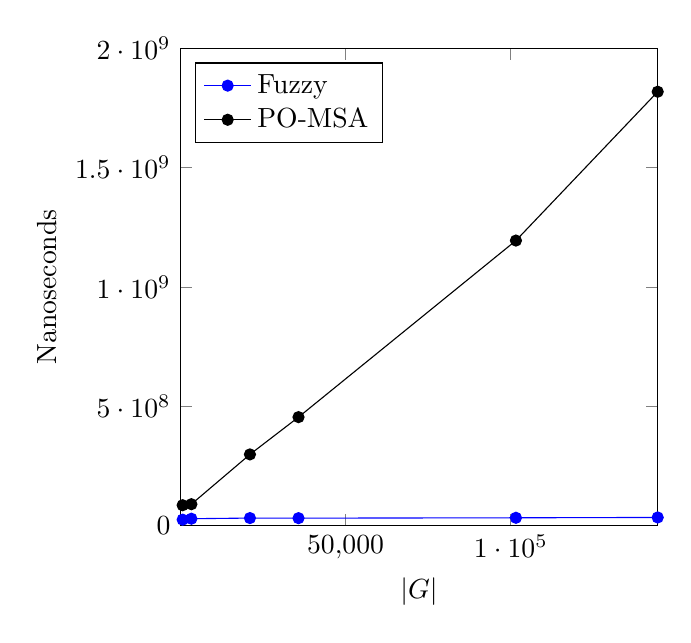
\begin{tikzpicture}
    \begin{axis}[scale only axis,height=0.5\textwidth,width=0.5\textwidth,xmin=0,ymin=0,xmax=144480,ymax=2000000000,scaled ticks=false, legend pos=north west, xlabel={$|G|$}, ylabel={Nanoseconds}, legend cell align=left, xtick={50000,100000,150000}]
      \addplot[color=blue,mark=*] coordinates {
        (700, 24601275)
        (3345, 28554977)
        (21070, 31282803)
        (35770,  30924263)
        (101570, 32429709)
        (144480, 33846424)
      };
      \addplot[color=black,mark=*] coordinates {
        (700, 85097029)
        (3345, 89367932)
        (21070, 297994542)
        (35770, 454186275)
        (101570, 1193934335)
        (144480, 1817456548)
      };
      \addlegendentry{Fuzzy}
      \addlegendentry{PO-MSA}
    \end{axis}
  \end{tikzpicture}
  \caption{Runtime of the alignment process as a function of $|G|$}
  \label{fig:runtime_G}
\end{figure}
\clearpage
\subsection*{Runtime as a function of error margin}
\textcolor{red}{GRAPH HAS VALUES FROM 3345 SIZE}
These tests are separated by varying the \texttt{-{}-error-margin} parameter. The results can be seen in figure \ref{fig:runtime_lambda}. The approach explodes in complexity as the number of allowed contexts increase exponentially. Already at \texttt{-{}-error-margin=1} the approach is slower than a regular PO-MSA search. Interestingly, we can see that the starting point for the exponential function is dependant on the graph sizes. When increasing the number of vertices to $150.000$ the approach is suddenly more efficient than PO-MSA up to $\lambda=2$ (Figure \ref{fig:runtime_lambda_large}). Additionally, if we utilize the parallellization through the \texttt{-{}-parallellization=true} we manage to put a linear bound on the exponential growth (Figure \ref{fig:runtime_lambda_parallell}).
\begin{figure}
  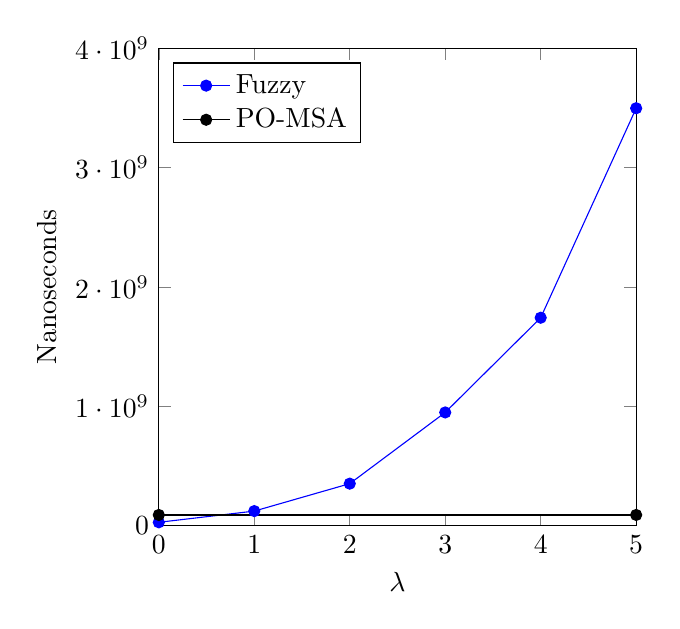
\begin{tikzpicture}
    \begin{axis}[scale only axis,height=0.5\textwidth,width=0.5\textwidth,xmin=0,ymin=0,xmax=5,ymax=4000000000,scaled ticks=false, legend pos=north west, xlabel={$\lambda$}, ylabel={Nanoseconds},xtick={0,1,2,3,4,5}, legend cell align=left]
      \addplot[color=blue,mark=*] coordinates {
        (0, 26977841)
        (1, 120987192)
        (2, 350870315)
        (3, 947601415)
        (4, 1741219879)
        (5, 3496580015)
      };
      \addplot[color=black,mark=*] coordinates {
        (0, 88628194)
        (5, 88628194)
      };
      \addlegendentry{Fuzzy}
      \addlegendentry{PO-MSA}
    \end{axis}
  \end{tikzpicture}
  \caption{Runtime of the alignment process as a function of $\lambda$}
  \label{fig:runtime_lambda}
\end{figure}
\begin{figure}
  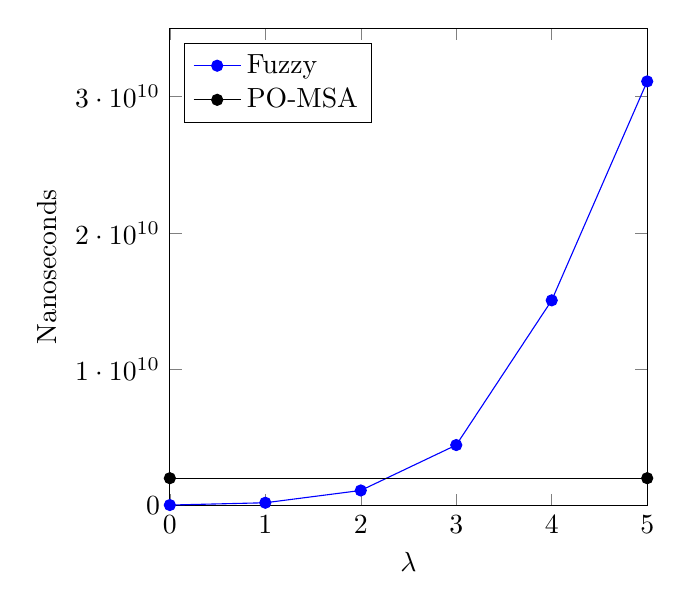
\begin{tikzpicture}
    \begin{axis}[scale only axis,height=0.5\textwidth,width=0.5\textwidth,xmin=0,ymin=0,xmax=5,ymax=35000000000,scaled ticks=false, legend pos=north west, xlabel={$\lambda$}, ylabel={Nanoseconds},xtick={0,1,2,3,4,5}, legend cell align=left]
      \addplot[color=blue,mark=*] coordinates {
        (0, 39421262)
        (1, 207661867)
        (2, 1109580502)
        (3, 4438734683)
        (4, 15048629538)
        (5, 31101186953)
      };
      \addplot[color=black,mark=*] coordinates {
        (0, 2008561551)
        (5, 2008561551)
      };
      \addlegendentry{Fuzzy}
      \addlegendentry{PO-MSA}
    \end{axis}
  \end{tikzpicture}
  \caption{Runtime of the alignment process as a function of $\lambda$ with $|G|=150.000$}
  \label{fig:runtime_lambda_large}
\end{figure}
\begin{figure}
  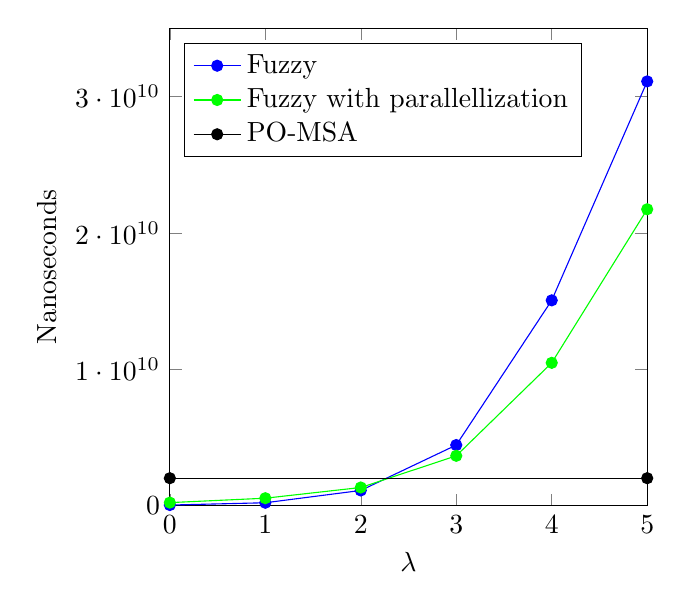
\begin{tikzpicture}
    \begin{axis}[scale only axis,height=0.5\textwidth,width=0.5\textwidth,xmin=0,ymin=0,xmax=5,ymax=35000000000,scaled ticks=false, legend pos=north west, xlabel={$\lambda$}, ylabel={Nanoseconds},xtick={0,1,2,3,4,5}, legend cell align=left]
      \addplot[color=blue,mark=*] coordinates {
        (0, 39421262)
        (1, 207661867)
        (2, 1109580502)
        (3, 4438734683)
        (4, 15048629538)
        (5, 31101186953)
      };
      \addplot[color=green,mark=*] coordinates {
        (0,217309155)
        (1,541668285)
        (2,1327223214)
        (3,3649467422)
        (4,10466121646)
        (5,21725713902)
      };
      \addplot[color=black,mark=*] coordinates {
        (0, 2008561551)
        (5, 2008561551)
      };
      \addlegendentry{Fuzzy}
      \addlegendentry{Fuzzy with parallellization}
      \addlegendentry{PO-MSA}
    \end{axis}
  \end{tikzpicture}
  \caption{Runtime of the alignment process as a function of $\lambda$ with $|G|=150.000$ and \texttt{-{}-parallellization=true}}
  \label{fig:runtime_lambda_parallell}
\end{figure}
\subsection*{Runtime as a function of sequence length}
Regulating sequence length is done by varying the \texttt{-{}-len} parameter sent to the read generator. The values used are approximations towards values found by actual sequencing technologies\cite{comparison_sequencing_systems}, the results can be found in table \ref{tab:runtimes_s}. As expected both algorithms are very linear with respect to read length, the fuzzy search growing seemingly slower than PO-MSA.
\begin{table}
  \begin{tabular}{|l|l|r|r|}
    \hline \textbf{Technology} & \textbf{Read length} & \textbf{PO-MSA time} & \textbf{Fuzzy time} \\ \hline
    HiSeq2000 (min) & 50 & 171961927 & 19347780 \\ \hline
    HiSeq2000 & 90 & 264031377 & 30038511 \\ \hline
    SOLiDv4 & 100 & 294027088 & 36927650 \\ \hline
    Ion PGM & 200 & 676355995 & 59767319 \\ \hline
    Sanger 3730xl (min) & 400 & 1117436847 & 98570092 \\ \hline
    454 GS FLX & 700 & 1600069004 & 167703497 \\ \hline
    Sanger 3730xl (max) & 900 & 2121961653 & 194846761 \\ \hline
  \end{tabular}
  \caption{Running times for different read lengths for the PO-MSA and fuzzy algorithms}
  \label{tab:runtimes_s}
\end{table}
\begin{figure}
  \begin{tikzpicture}
    \begin{axis}[scale only axis,height=\textwidth,width=\textwidth,xmin=0,ymin=0,xmax=900,ymax=2500000000,scaled ticks=false, legend pos=north west, xlabel={$\lambda$}, ylabel={Nanoseconds}, legend cell align=left]
      \addplot[color=blue,mark=*] coordinates {
        (50,19347780)
        (90,30038511)
        (100,36927650)
        (200,59767319)
        (400,98570092)
        (700,167703497)
        (900,194846761)
      };
      \addplot[color=black,mark=*] coordinates {
        (50,171961927)
        (90,264031377)
        (100,294027088)
        (200,676355995)
        (400,1117436847)
        (700,1600069004)
        (900,2121961653)
      };
      \addlegendentry{Fuzzy}
      \addlegendentry{PO-MSA}
    \end{axis}
  \end{tikzpicture}
  \caption{Runtime of the alignment process as a function of $|s|$}
  \label{fig:runtime_s}
\end{figure}
\subsection*{Runtime as a function of graph complexity}
\subsection*{Correctness as a function of noise}
There are two reasons for running these tests: Finding bugs in the tool and learning about statistical distributions. The approach is shown to be correct whenever $\lambda$ is greater than the edit distance to the most similar path in the graph, and wrong when it is not. These results are thus an projection of the probability of generating a read $r$ such that $\lambda>=maxscore(r)$ given an error probability $p$. We do however include these results as they reflect usage in an everyday, non-controlled environment. For the first set of tests we set $\lambda=2$, as this is the cutoff-point where a fuzzy search is still more efficient than PO-MSA. The results can be seen in table \ref{tab:correctness}
\begin{wraptable}{r}{0.3\textwidth}
  \begin{tabular}{|c|c|}
    \hline $p$ & \textbf{Correctness} \\ \hline
    0.00 & 100\% \\ \hline
    0.01 & 90\% \\ \hline
    0.02 & 60\% \\ \hline
    0.04 & 60\% \\ \hline
    0.06 & 40\% \\ \hline
    0.08 & 20\% \\ \hline
    0.1 & 10\% \\ \hline
  \end{tabular}
  \caption{Percentage of correctly aligned reads as $p$ varies and $\lambda$ is fixed}
  \label{tab:correctness}
\end{wraptable}
A more interesting experiment is looking at the correctness while both varying $p$ and $\lambda$. In table \ref{fig:correctness_both} we can see the results from such an experiment. Every cell represents the number of correct runs out of 100 tests, which conveniently is equivalent to the error percentage. Every row represents one table corresponding to table \ref{tab:correctness}. More interestingly, every column corresponds to a single mutation-probability which would typically be correlated with an entire data-set. Although the sample is small there seems to be a trend where the number of correctly mapped reads logarithmically increases as the error-margin is increased.
\begin{figure}
  \begin{center}
    \begin{tikzpicture}[every node/.style={anchor=base,text depth=.5ex,text height=2em,text width=2em},align=center,text centered]
      \matrix(A) [nodes={rectangle}] {
        \node {5}; & \HeatmapNode{100} & \HeatmapNode{100} & \HeatmapNode{99} & \HeatmapNode{96} & \HeatmapNode{83} & \HeatmapNode{80} \\
        \node {4}; & \HeatmapNode{100} & \HeatmapNode{99} & \HeatmapNode{96} & \HeatmapNode{83} & \HeatmapNode{73} & \HeatmapNode{61} \\
        \node {3}; & \HeatmapNode{100} & \HeatmapNode{97} & \HeatmapNode{87} & \HeatmapNode{76} & \HeatmapNode{52} & \HeatmapNode{45} \\
        \node {2}; & \HeatmapNode{100} & \HeatmapNode{93} & \HeatmapNode{73} & \HeatmapNode{59} & \HeatmapNode{44} & \HeatmapNode{41} \\
        \node {1}; & \HeatmapNode{100} & \HeatmapNode{84} & \HeatmapNode{55} & \HeatmapNode{38} & \HeatmapNode{36} & \HeatmapNode{25} \\
        \node {0}; & \HeatmapNode{100} & \HeatmapNode{79} & \HeatmapNode{38} & \HeatmapNode{18} & \HeatmapNode{10} & \HeatmapNode{4} \\
        \node {};  & \node{0}; & \node{0.01}; & \node{0.02}; & \node{0.03}; & \node{0.04}; & \node{0.05}; \\
      };
      \node[draw=none] at (0.5, -0.75) {$p$};
      \node[draw=none] at (-4, 3.85) {$\lambda$};
    \end{tikzpicture}
  \end{center}
  \caption{Percentage of correctly aligned reads as a function of both $p$ and $\lambda$ varies}
  \label{fig:correctness_both}
\end{figure}
\section{Comparison with other tools}
\label{sec:comparison_tools}
\end{document}